% \subsection{問題設定}
% 本研究では,銀行のローンの審査システムについての機械学習モデルを想定し,認可拒否について誤分類を引き起こす敵対的サンプルを生成することを考える.銀行のローンを申請する顧客情報と正解データをもとに機械学習モデルが学習し,テストデータに対する分類結果を出力する.敵対的サンプルによる誤分類は,銀行にとってリスクの高いローンを誤って認可してしまう可能性がある.このような問題に対処するため,機械学習モデルの安全性が求められており,敵対的サンプルに対する防御手法が必要である.また同時に,モデルの脆弱性を理解することは,安全性を向上させるために重要である.

\subsection{敵対的学習}
敵対的学習は,機械学習モデルの堅牢性を向上させるための手法として誕生した.従来の機械学習モデルは,訓練データに対して高い精度を示す一方で,敵対的サンプルと呼ばれる微細ななノイズを含むデータに対しては脆弱である
ことが知られている.これにより,モデルが誤分類を引き起こし,セキュリティ上のリスクが生じる可能性がある.

goodfellowらの研究\cite{goodfellow2015explaining}でこの敵対的学習について提案された.この手法では,正常データと敵対的サンプルの特徴をAIに学習させる防御手法である.機械学習モデルの学習時において,正常データと敵対的サンプルに対する誤差(Loss)をそれぞれ計算し,これらを足し合わせた値を基のモデルの重み $\bm{w}$ を更新することで,敵対的サンプルの特徴を学習する.

以下に実際の敵対的学習の流れを示す.\cite{MBSD-AdversarialTraining}

\begin{enumerate}

    \item 学習中の機械学習モデルを利用して敵対的サンプルを作成する

    元データの画像を機械学習モデルに入力し,予測ラベル $y$ を得る.また,この予測と正解データを比較した誤差を $Loss$ 関数で計算し,この誤差を最小化するように敵対的サンプルを生成する.
    
    \begin{figure}[H]
        \centering
        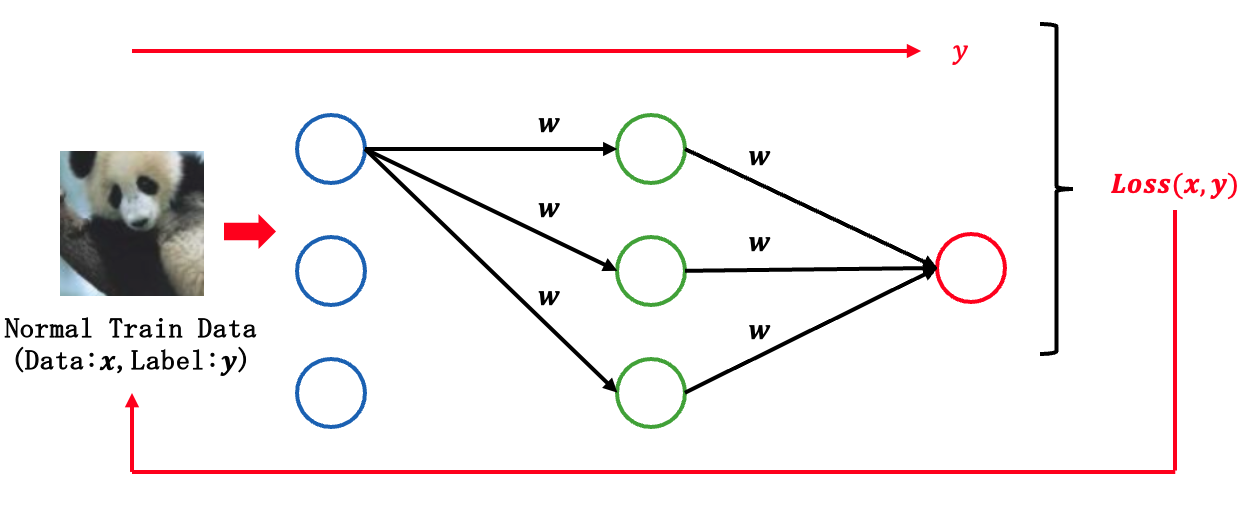
\includegraphics[width=0.8\textwidth]{images/敵対的学習1.png}
        \caption{敵対的学習1:元データによる}
        \label{fig:adversarial_learning1}
    \end{figure}
    
    \item 機械モデルに正常なデータ $\bm{x}$ と敵対的サンプル $\bm{x}'$ を入力し,それぞれの誤差 $Loss$ を得る

    図2の上の画像が元データで下の画像が先ほどノイズを加えた画像である.それぞれ機械学習モデルに入力し,それぞれの誤差を取得する.

    \begin{figure}[H]
        \centering
        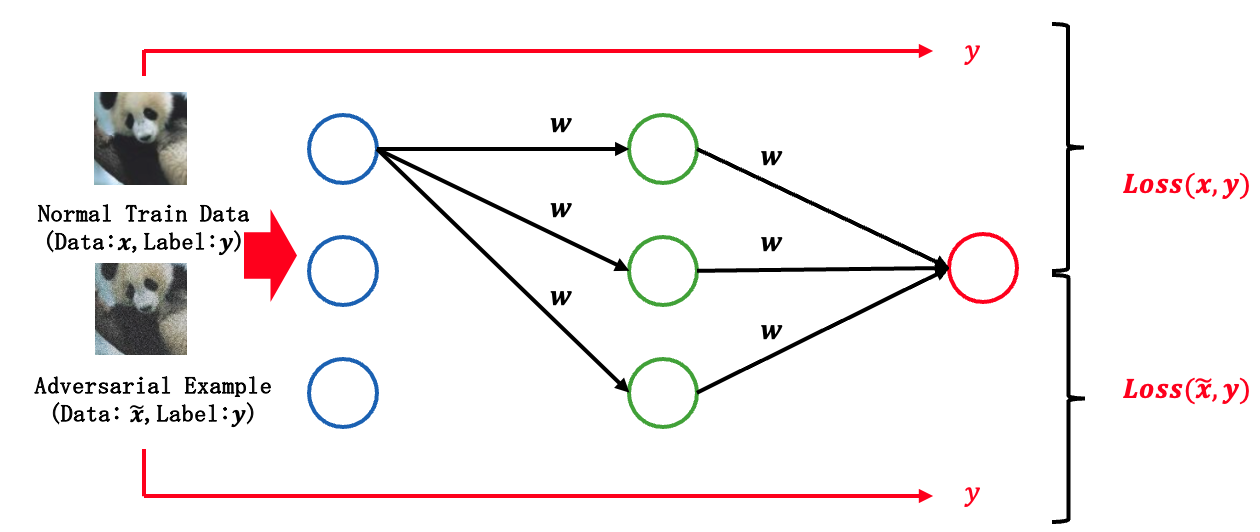
\includegraphics[width=0.8\textwidth]{images/敵対的学習2.png}
        \caption{敵対的学習2:元データと敵対敵サンプルの誤差を取得する}
        \label{fig:adversarial_learning2}
    \end{figure}

    \item それぞれ得た誤差 $Loss(x, y), Loss(x', y)$ に重み係数 $\alpha$ をつけて足し合わせる

    元データと敵対的サンプル両方の誤差を取得し,重み $\alpha$ をつけて足し合わせることで,敵対的サンプルの挙動のバランスを以下の式(1)で調整できる.
    \autoequation{\alpha \cdot Loss(x,y)+(1−\alpha) \cdot Loss(\tilde{x},y)}
    \begin{figure}[H]
        \centering
        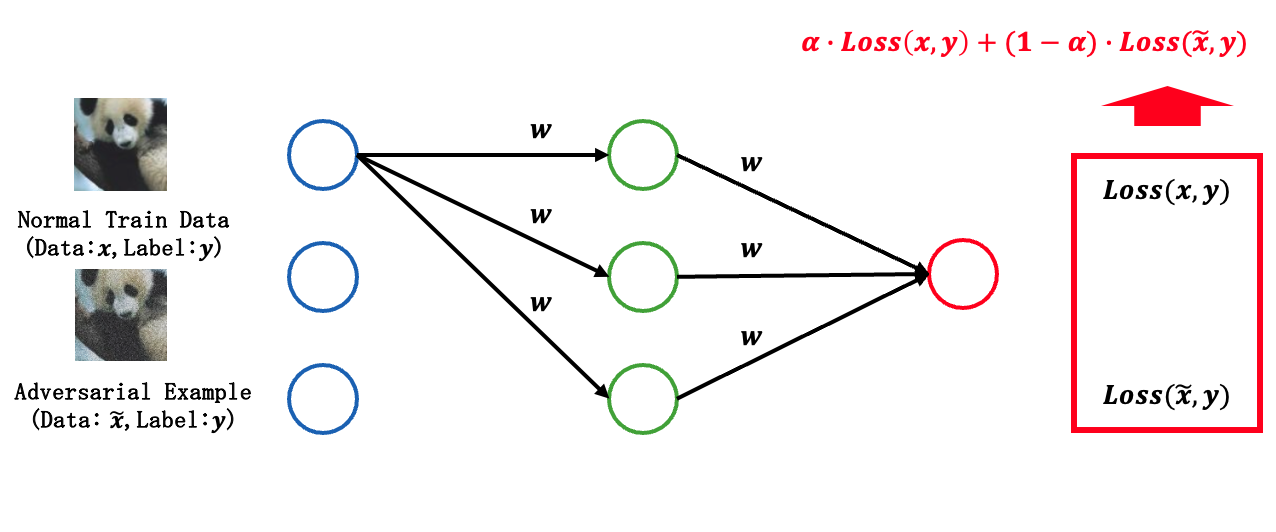
\includegraphics[width=0.8\textwidth]{images/敵対的学習3.png}
        \caption{敵対的学習3:元データと敵対敵サンプルの誤差を足し合わせる}
        \label{fig:adversarial_learning3}
    \end{figure}

    \item 足し合わされた誤差 $Loss$ が最小となるように,重み $\bm{w}$ を更新する

    図1で学習された機械学習モデルの重み $w$ を敵対的サンプルに対応させるため更新する.
    先ほどの式(1)を最小化することで,重み $w$ を $w_{\_new}$ に更新する.これにより,敵対的サンプルの挙動を抑えることができた機械学習モデルを作成することができる.
    
    \begin{figure}[H]
        \centering
        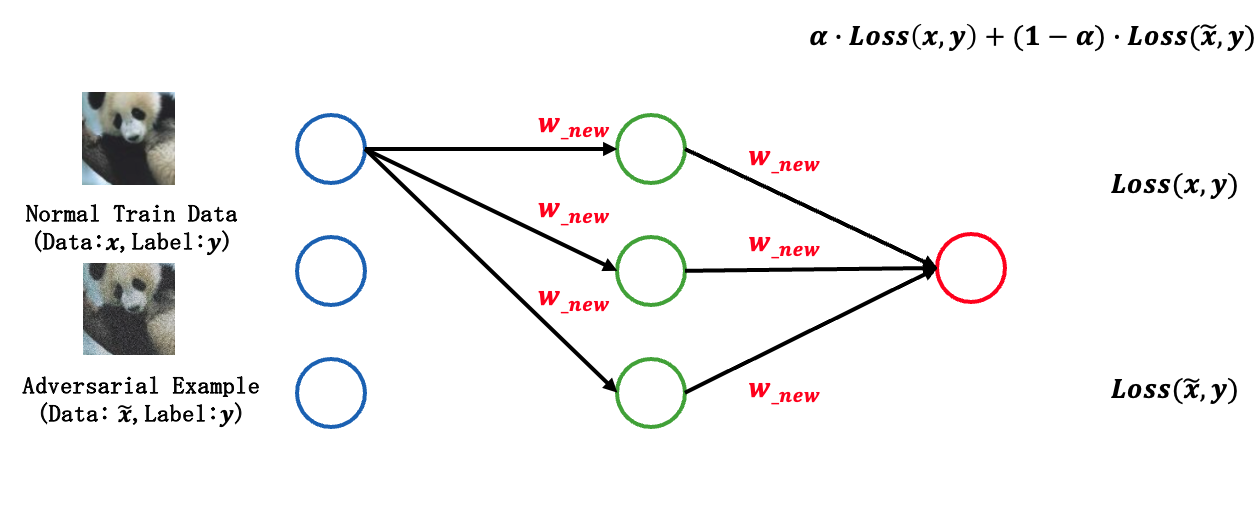
\includegraphics[width=0.8\textwidth]{images/敵対的学習4.png}
        \caption{敵対的学習4:足し合わされた誤差が最小となるよう重みを更新する}
        \label{fig:adversarial_learning4}
    \end{figure}

\end{enumerate}

以上の流れにより,敵対的学習を行うことで,機械学習モデル敵対的サンプルの挙動に対応することができ,堅牢性を向上させることができる.

\subsection{敵対的サンプル}
先ほどの敵対的学習の説明の中の一番最初のステップで生成した敵対的サンプルについて説明する.改めて敵対的サンプルとは,人間には見分けのつかない微細なノイズをデータに付与することで機械学習モデルの誤分類を引き起こすデータである.\cite{MBSD-AdversarialExample}運用している機械学習モデルを狙った攻撃に使用されることがある.

敵対的サンプルによる誤分類を確認した実験をGoodfellowらが行っている\cite{goodfellow2015explaining}.
\begin{figure}[H]
    \centering
    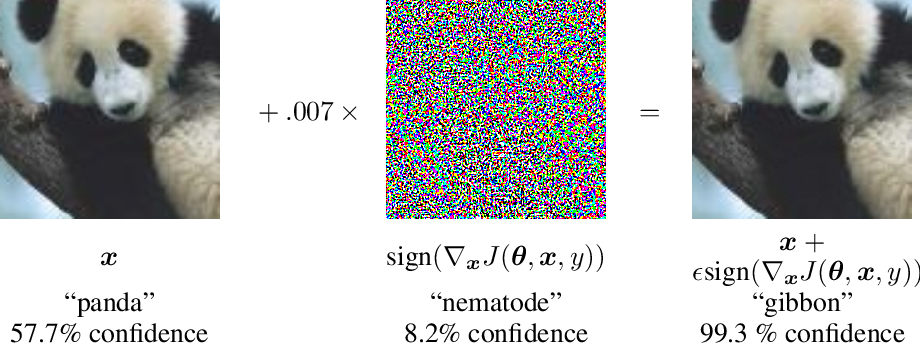
\includegraphics[width=0.8\textwidth]{images/goodfellow_panda.png}
    \caption{敵対的サンプルの例:パンダの敵対的サンプル画像によってテナガザルと誤分類する\cite{goodfellow2015explaining}}
    \label{fig:adversarial_example}
\end{figure}

この研究では,様々な動物に関する画像を学習した機械学習モデルに対して,人間には見分けがつかない微細なノイズを付与したパンダの画像を入力するとテナガザルと誤分類されることを示した.

このような画像データに対する敵対的サンプルの生成は行うことができる.しかし,表形式データに対する敵対的サンプルは,先ほどの手法を用いて生成することは難しい.その理由として,表形式データの特徴量は画像データと異なる性質を持つためである.画像データの場合,各ピクセルの値は0から255の範囲の連続値として扱うことができ,わずかな変化は人間の目では認識できないことが多い.一方で,表形式データの特徴量には,年齢や収入といった数値データだけでなく,性別や職業といったカテゴリカル変数も含まれる.また,各特徴量は独立した意味を持っており,それぞれの特徴量の変化は明確な意味の変化を伴う.例えば,先ほどのパンダの画像の場合,個々のピクセル値にわずかな変化を加えても,人間にとってはそれが「パンダの画像」であることに変わりはない.しかし,ローン申請データにおいて,年収を示す特徴量に対してわずかな変化を加えた場合,その変化は申請者の経済状況を直接的に変えてしまう可能性がある.さらに,職業などのカテゴリカルデータの場合,わずかな変化という概念自体が適用できない.このような表形式データの特性により,画像データに対する敵対的サンプル生成手法をそのまま適用することは適切ではない.そこで,表形式データの特性を考慮した新たな敵対的サンプル生成手法が必要となる.特に,各特徴量の重要度や,特徴量の種類(連続値かカテゴリカル値か)を考慮した手法が求められる.


\subsection{使用するデータセット}
今回使用するデータは,OpenMLが提供しているドイツにおける信用情報データセットcredit-gである.このデータセットは,ドイツの銀行の顧客情報を元に,ローンの信用リスクを予測するためのデータセットである.このデータセットで使用した特徴量は,以下の通りである.

\begin{table}[H]
    \centering
    \caption{信用情報データセットの特徴量}
    \begin{tabular}{|l|l|l|}
        \hline
        特徴量名 & 意味 & 種類 \\ \hline
        checking\_status & 既存の当座預金口座のステータス(ドイツマルク) & カテゴリ \\ \hline
        duration & 期間(月) & 数値 \\ \hline
        credit\_amount & クレジットの金額(申請する与信金額) & 数値 \\ \hline
        savings\_status & 貯蓄口座/債券のステータス(ドイツマルク建て) & カテゴリ \\ \hline
        employment & 現在の雇用年数 & カテゴリ \\ \hline
        installment\_commitment & 可処分所得に対する分割払いの割合 & 数値 \\ \hline
        residence\_since & X年からの現在の居住地 & 数値 \\ \hline
        age & 年齢 & 数値 \\ \hline
        existing\_credits & この銀行の既存クレジット数 & 数値 \\ \hline
        num\_dependents & 扶養家族数 & 数値 \\ \hline
        own\_telephone & 電話 & カテゴリ \\ \hline
        foreign\_worker & 外国人労働者 & カテゴリ \\ \hline
        target & ローン承認 (true) or ローン却下(false) & カテゴリ \\ \hline
    \end{tabular}
    \label{tab:credit_g_features}
\end{table}

カテゴリ変数についてはダミー変数化し離散値として扱う.また数値の特徴量についても全て離散値であることがわかった.このデータセットは,ローンの信用リスクを予測するためのデータセットであるため,ローンの承認結果を予測する二値分類問題として扱う.